\section{参数敏感性}
\label{sec:opt-con-sensitivity}

章首问过：预算从$2$增加到$2.1$，最优值会下降多少？这类问题改变的是问题数据，而不是求解过程。本节固定建模形式，让约束右端或其他参数变化，分别研究两个输出：最优值怎样变，最优解怎样变。二者需要的条件不同：最优值的变化可以由对偶乘子给出可靠的单侧界，即使值函数不可微；最优解的变化则要求KKT方程组在参数附近有可微的解分支。

\subsection{最优值的变化}
\label{sec:opt-con-value-sensitivity}

\paragraph{乘子给出的支撑界}
把约束的右端放松为参数，考虑
\begin{equation}
\label{eq:opt-con-perturbed}
  p(\bm u,\bm v)=\inf\{f(\bm x):g_i(\bm x)\leq u_i,\ h_j(\bm x)=v_j\},
\end{equation}
不可行时记$p=+\infty$。$\bm u_i>0$表示放宽第$i$条不等式，$u_i<0$表示收紧。上一节的扰动值函数就是这个函数在$\bm v=\bm0$时的情形。

\begin{theorem}[最优值的全局支撑界]
\label{thm:opt-con-global-sensitivity}
设未扰动问题的强对偶成立，且对偶最优值被$(\bm\lambda^\star,\bm\nu^\star)$达到。则对所有$(\bm u,\bm v)$，
\begin{equation}
\label{eq:opt-con-sensitivity-bound}
  p(\bm u,\bm v)\geq p(\bm0,\bm0)-\langle\bm\lambda^\star,\bm u\rangle-\langle\bm\nu^\star,\bm v\rangle.
\end{equation}
\end{theorem}

\begin{proof}
若扰动问题不可行，左端为$+\infty$，结论成立。否则任取扰动问题的可行点$\bm x$。由$\bm\lambda^\star\geq\bm0$、$g_i(\bm x)\leq u_i$、$h_j(\bm x)=v_j$，
\[
  p(\bm0,\bm0)=q(\bm\lambda^\star,\bm\nu^\star)\leq\mathcal L(\bm x,\bm\lambda^\star,\bm\nu^\star)\leq f(\bm x)+\langle\bm\lambda^\star,\bm u\rangle+\langle\bm\nu^\star,\bm v\rangle.
\]
移项后对可行$\bm x$取下确界即得。
\end{proof}

这个界只用到强对偶与对偶达到，不要求原问题凸，也不要求$p$可微；它对任意大小的扰动都成立，只是方向是单侧的。读法如下：收紧第$i$条约束（$u_i<0$）时，最优值至少增加$\lambda_i^\star|u_i|$，所以大乘子提示这条约束一收紧代价就很高；放宽它（$u_i>0$）时，最优值至多下降$\lambda_i^\star u_i$，但实际下降可能更少。这与第~\ref{chap:opt-linear-programming}章固定最优基时对偶变量作为资源价格的解释一致；线性规划中只要最优基不变，界就取等号，换基后才出现偏差。

回到章首：预算分配例在$\tau=2$时乘子$\lambda_1^\star=1/2$，最优值$V(2)=1/4$。预算约束写成$x_1+x_2-2\leq u$，$u=\tau-2$。界~\eqref{eq:opt-con-sensitivity-bound}给出$V(\tau)\geq\frac14-\frac12(\tau-2)$。直接计算可知$1\leq\tau\leq3$时$V(\tau)=(3-\tau)^2/4$，于是$V(2.2)=0.16\geq0.15$，$V(1.8)=0.36\geq0.35$。预算增加$0.1$时，最优值至多下降$0.05$，实际下降$0.25-0.2025=0.0475$。

\paragraph{乘子何时是导数}
如果$p$恰好在$(\bm0,\bm0)$处可微，界~\eqref{eq:opt-con-sensitivity-bound}立刻给出导数：函数$\varphi(\bm u,\bm v)=p(\bm u,\bm v)-p(\bm0,\bm0)+\langle\bm\lambda^\star,\bm u\rangle+\langle\bm\nu^\star,\bm v\rangle$非负且在原点为零，原点是它的最小点，可微时梯度为零，于是
\begin{equation}
\label{eq:opt-con-multiplier-derivative}
  \frac{\partial p}{\partial u_i}(\bm0,\bm0)=-\lambda_i^\star,\qquad
  \frac{\partial p}{\partial v_j}(\bm0,\bm0)=-\nu_j^\star.
\end{equation}
预算分配例中$V'(\tau)=-(3-\tau)/2=-\lambda_1^\star(\tau)$，在$\tau=2$处为$-1/2$。图~\ref{fig:opt-con-sensitivity}(a)画出$V(\tau)$和乘子曲线：红色点线是$\tau=2$处斜率为$-1/2$的支撑直线，整条曲线位于它的上方；$\tau\geq3$时预算不再限制解，乘子为零，$V$保持为零；$0<\tau<1$时第二个非负约束也活跃，$V(\tau)=((2-\tau)^2+1)/2$，乘子为$2-\tau$。三段在$\tau=1$与$\tau=3$处衔接时乘子连续，所以$V$仍然可微，只是二阶导数跳变。

可微性不能省略。考虑$\min-x$、约束$x\leq b$与$x\leq1$。当$b<1$时$V(b)=-b$，当$b>1$时$V(b)=-1$，即$V(b)=\max\{-b,-1\}$。在$b=1$处两条约束都活跃，驻点方程$-1+\lambda_1+\lambda_2=0$允许任意$\lambda_1\in[0,1]$、$\lambda_2=1-\lambda_1$，乘子不唯一。每个$\lambda_1$都给出一条斜率为$-\lambda_1$的支撑直线（图~\ref{fig:opt-con-sensitivity}(b)），所以无论向哪一侧改变$b$，界~\eqref{eq:opt-con-sensitivity-bound}都可靠；但$V$的左导数为$-1$、右导数为$0$，没有唯一的一阶变化率。多重乘子与值函数折点在这里同时出现：全部最优乘子的负值恰好组成$V$在折点处所有支撑斜率的集合$[-1,0]$。

\begin{figure*}[!htbp]
  \centering
  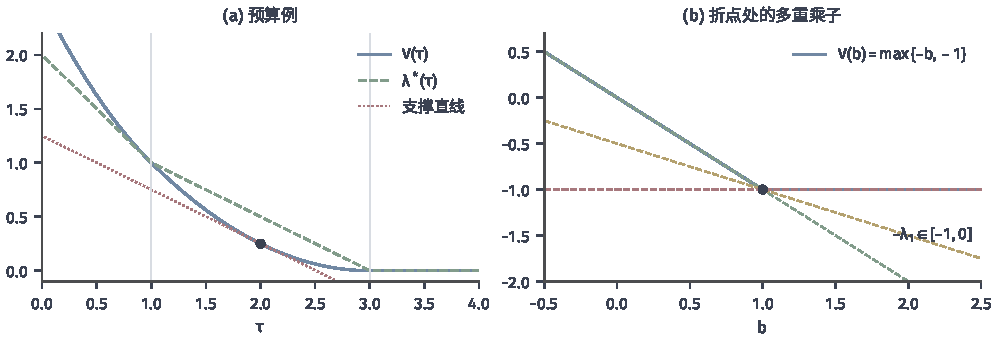
\includegraphics[width=169mm]{figures/03-optimization-evolution-and-signals/01-optimization/matplotlib/c5-sensitivity/figure.pdf}
  \caption{最优值随约束右端的变化。(a) 预算分配例：蓝线为最优值$V(\tau)$，绿色虚线为预算乘子$\lambda^\star(\tau)$，红色点线为$\tau=2$处斜率$-1/2$的支撑直线，灰色竖线标出活动集改变的$\tau=1,3$。(b) $\min-x$、$x\leq b$、$x\leq1$：$V(b)=\max\{-b,-1\}$在$b=1$处有折点，斜率$-1,-0.5,0$的三条虚线都是合法的支撑直线，对应不同的最优乘子。}
  \label{fig:opt-con-sensitivity}
\end{figure*}

\subsection{最优解的变化}
\label{sec:opt-con-solution-sensitivity}

最优值是一个数，最优解是一个向量，后者的变化需要更多结构。下面设目标与约束依赖参数$\theta$，且在$\theta_0$处有一个KKT点$(\bm x_0,\bm\lambda_0,\bm\nu_0)$。

\paragraph{固定活动集的KKT方程组}
设活动集为$I$，并且活跃约束的乘子都为正、未活跃约束严格满足（称为严格互补）。若参数变化后活动集保持为$I$，未活跃约束和它们的零乘子可以暂时忽略，解由下列方程组决定：
\[
  \bm F(\bm x,\bm\lambda_I,\bm\nu,\theta)=
  \begin{bmatrix}
    \nabla_{\bm x}\mathcal L(\bm x,\bm\lambda_I,\bm\nu,\theta)\\
    \bm g_I(\bm x,\theta)\\
    \bm h(\bm x,\theta)
  \end{bmatrix}=\bm0.
\]
记$\bm J$为活跃约束与等式约束的Jacobian（行为$\nabla g_i^\top$、$\nabla h_j^\top$），$\bm H=\nabla^2_{\bm x\bm x}\mathcal L$。方程组关于$(\bm x,\bm\lambda_I,\bm\nu)$的Jacobian是KKT矩阵
\begin{equation}
\label{eq:opt-con-kkt-matrix}
  \bm K=\begin{bmatrix}\bm H&\bm J^\top\\\bm J&\bm0\end{bmatrix}.
\end{equation}
若$\bm K$在$\theta_0$处可逆，隐函数定理（\BookChapterRef{chap:multivariate-calculus}{卷一“多元函数微分”章}）给出$\theta_0$附近唯一的连续可微解分支，导数由线性方程$\bm K\,\mathrm d(\bm x,\bm\lambda_I,\bm\nu)/\mathrm d\theta=-\partial\bm F/\partial\theta$确定。严格互补与连续性保证$\theta$足够接近$\theta_0$时活跃乘子仍为正、未活跃约束仍严格满足，因此这一分支确实是扰动问题的KKT点。

\begin{lemma}[KKT矩阵可逆的充分条件]
\label{lem:opt-con-kkt-matrix}
若$\bm J$行满秩（即LICQ），且$\bm H$在零空间$\ker\bm J$上正定（对所有非零$\bm d$，$\bm J\bm d=\bm0$蕴含$\bm d^\top\bm H\bm d>0$），则$\bm K$可逆。
\end{lemma}

\begin{proof}
设$\bm H\bm d+\bm J^\top\bm w=\bm0$、$\bm J\bm d=\bm0$。用$\bm d^\top$左乘第一式得$\bm d^\top\bm H\bm d=-(\bm J\bm d)^\top\bm w=0$，由零空间上的正定性得$\bm d=\bm0$；于是$\bm J^\top\bm w=\bm0$，行满秩给出$\bm w=\bm0$。
\end{proof}

预算分配例在$1<\tau<3$时活动集为$\{1\}$，$\bm H=\bm I$，$\bm J=(1,1)$。方程组为$\bm x-\bm c+\lambda(1,1)^\top=\bm0$、$x_1+x_2-\tau=0$，对$\tau$求导得$\bm x'+\lambda'(1,1)^\top=\bm0$、$x_1'+x_2'=1$，解出$\bm x'=(1/2,1/2)^\top$、$\lambda'=-1/2$，与显式解$\bm x^\star(\tau)=((\tau+1)/2,(\tau-1)/2)^\top$一致。

约束梯度独立本身并不保证$\bm K$可逆。最小化$\frac12x_2^2$、约束$x_2-\theta=0$，变量为$(x_1,x_2)$。约束梯度$(0,1)^\top$非零，LICQ成立；但$\bm H=\operatorname{diag}(0,1)$在$\ker\bm J=\{(t,0)^\top\}$上为零，$\bm K$奇异。对应地，解集$\{(x_1,\theta)^\top:x_1\in\mathbb R\}$是一条直线，“最优解对$\theta$的导数”根本没有确定的含义。

\paragraph{局部描述何时失效}
固定活动集的分析只在一个区间内有效。预算分配例在$\tau=1$与$\tau=3$处改变活动集：$\tau$跨过$3$时预算约束从带正乘子变为不起作用，$\bm x^\star(\tau)$的导数从$(1/2,1/2)^\top$跳到$\bm0$；跨过$1$时第二个非负约束开始活跃，导数跳到$(1,0)^\top$。在切换点，严格互补不成立（例如$\tau=3$时活跃约束的乘子为零），解仍然连续，但不可微。

局部驻点分支也不自动代表全局最优解。考虑$\min_x(x^2-1)^2+\theta x$。$\theta=0$时有两个全局最小点$\pm1$。驻点方程$4x(x^2-1)+\theta=0$在$(x,\theta)=(1,0)$处关于$x$的导数为$12x^2-4=8\neq0$，隐函数定理给出光滑分支$x(\theta)$，$x'(0)=-1/8$；在$-1$附近也有一条同样的分支。两条分支都是局部最小点，但$\theta>0$时$\theta x$项使$-1$附近的分支取更低的值，$\theta<0$时则相反。沿着$+1$分支计算导数是正确的，但这条分支在$\theta>0$时已不再是全局最优解；全局最优解在$\theta=0$处从一条分支跳到另一条，最优值的一阶近似为$-|\theta|$，出现折点。

最后，本节研究的是模型改变后\emph{精确}最优解和最优值的变化，与在同一问题上迭代截断、舍入或内层近似求解造成的误差是两回事。前者由KKT矩阵、活动集与乘子决定，后者由算法的收敛速度与停止规则决定。报告结果时应分开说明：数据扰动$\Delta\theta$通过导数或支撑界影响多少，计算误差又由残差或间隙证书控制到多少。二者都可能主导最终误差，却不能互相代替。
